\section{Синтаксический анализ графов}
В данном разделе будут даны основные определения из области синтаксического анализа графов, и рассмотрены различные формулировки задач этой области с использованием контекстно-свободных грамматик.

В данной работе пустую строку будем обозначать $\varepsilon$, а конкатенацию двух строк $S_{1}$ и $S_{2}$~--- $S_{1} \cdot S_{2}$.

\begin{mydef}
Граф --- это тройка $G = (Q,\Sigma,\delta)$, где $Q \cap \Sigma =  \emptyset$, $Q$~--- конечное множество вершин графа, $\Sigma$~--- конечный алфавит символов, используемых в качестве меток на ребрах графа, и $\delta \subseteq Q \times \Sigma \times Q$~--- конечное множество ребер, помеченных символами из $\Sigma$.
\end{mydef}
Если $m \in Q$ и $\sigma \in \Sigma$, тогда $\delta(m,\sigma) = \{n~|~(m, \sigma, n) \in \delta\}$ обозначает множество вершин графа, которые имеют входящее ребро из вершины $m$, помеченное символом $\sigma$. Если $m \in Q$ и $S \in \Sigma^*$, то


\[ \delta^*(m, S) =
  \begin{cases}
    \{m\}       & \quad \text{if } S = \varepsilon ;\\
    \cup_{n \in \delta(m, \sigma)} \delta^*(n, S')  & \quad \text{if } S = \sigma \cdot S'.\\
  \end{cases}
\]

Язык, который порождается графом $G$ и выделенными в нем вершинами $m, n \in Q$, обозначим $L(G, m, n)$, где
\[ L(G, m, n) = \{S \in \Sigma^*~|~n \in \delta^*(m, S)\}.
\]

В дальнейшем будут рассматриваться контекстно-свободные грамматики, которые находятся в нормальной форме Хомского~\cite{azimov-spbu-binChomsk}, и в которых исключается вывод пустой строки. Для простоты представления введем следующее определение.

\begin{mydef}
Контекстно-свободная грамматика --- это тройка $C = (N,\Sigma,P)$, где $N \cap \Sigma =  \emptyset$, $N$ --- конечное множество нетерминалов грамматики, $\Sigma$ --- конечный алфавит символов, $P$ --- множество правил грамматики. Кроме того, все правила грамматики записываются в одной из следующих форм: $a \rightarrow b~c$ или $a \rightarrow \sigma$, где $a,b,c \in N$ и $\sigma \in \Sigma$.
\end{mydef}

В данном определении не указывается стартовый нетерминал грамматики, поэтому для определения языка, порождаемого данной грамматикой, необходимо указать соответствующий нетерминал. Тогда язык, порождаемый грамматикой $C$, со стартовым нетерминалом $a \in N$ обозначим $L(C,a)$.

В контексте задач синтаксического анализа графов бывает необходимо отвечать на различного рода вопросы, связанные с искомыми в графе путями. Тип вопросов, на которые отвечает задача принято называть \textit{семантикой запроса}. Далее сформулируем задачи синтаксического анализа графов с использованием КС-грамматики $C$ и различных семантик запросов, рассмотренных в работах~\cite{azimov-spbu-hellings1, azimov-spbu-hellings2}.

Использование \textit{relational} семантики запроса означает, что для нетерминала $a \in N$ и графа $G$ необходимо построить множество $\{(m, n)~|~L(C,a) \cap L(G,m,n) \neq \emptyset \}$.

Использование \textit{all-path} семантики запроса означает, что для нетерминала $a \in N$, графа $G$ и его вершин $m,n \in Q$, необходимо предъявить все пути из вершины $m$ в вершину $n$, такие что метки на ребрах этих путей образуют строку из языка $L(C,a)$.

Использование \textit{single-path} семантики запроса означает, что для нетерминала $a \in N$, графа $G$ и его вершин $m,n \in Q$, необходимо предъявить какой-нибудь путь (если он существует) из вершины $m$ в вершину $n$, такой что метки на ребрах этого пути образуют строку из языка $L(C,a)$.

В качестве грамматики, порождающей язык $L(C,a) \cap L(G,m,n)$, в работе~\cite{azimov-spbu-hellings2} используется \textit{аннотированная грамматика}, определенная следующим образом.

\begin{mydef}
Пусть имеется КС-грамматика $C = (N,\Sigma,P)$ и граф $G = (Q,\Sigma,\delta)$. Тройки $(a,m,n) \in N \times Q \times Q$ будем обозначать $a[m,n]$. Тогда аннотированная грамматика --- это КС-грамматика $C_{G} = (N_{G}, \Sigma, P_{G})$, в которой $N_{G} \subseteq N \times Q \times Q$; каждое правило из $P_{G}$ вида $a[m,n] \rightarrow b[m,o]~c[o,n]$ или вида $a[m,n] \rightarrow \sigma$, где $a,b,c \in N$, $m, n, o \in Q$ и $\sigma \in \Sigma$; и выполняются следующие три правила:

\begin{enumerate}
\item $a[m,n] \in N_{G} \Leftrightarrow L(C,a) \cap L(G,m,n) \neq \emptyset$,
\item $(a[m,n] \rightarrow b[m,o]~c[o,n]) \in P_{G} \Leftrightarrow (a \rightarrow b~c) \in P$,
\item $(a[m,n] \rightarrow \sigma) \in P_{G} \Leftrightarrow (m, \sigma, n) \in \delta \wedge (a \rightarrow \sigma) \in P$.
\end{enumerate}

\end{mydef}

\section{Конъюнктивные грамматики}
В работе будут рассматриваться конъюнктивные грамматики~\cite{azimov-spbu-conj}, которые представляют собой расширение контекстно-свободных грамматик операцией пересечения.

\begin{mydef}
Конъюнктивная грамматика~--- это четверка $C =$ \\ $(\Sigma, N, P, S)$, где $N \cap \Sigma =  \emptyset$, $N$~--- конечное множество нетерминалов грамматики, $\Sigma$~--- конечный алфавит символов, $P$~--- множество правил грамматики, а $S$~--- стартовый нетерминал. Кроме того, все правила грамматики имеют вид $a \rightarrow \alpha_{1}~\& \ldots \&~\alpha_{n}$, где $a \in N$, $\alpha_{i} \in (\Sigma \cup N)^*$, $n \ge 1$.
\end{mydef}

Язык, порождаемый конъюнктивной грамматикой, определяется с помощью вывода, в котором на каждом шаге выполняется одно из двух действий:
\begin{itemize}
    \item нетерминал заменяется телом правила, заключенным в скобки;
    \item подстрока вида $(w~\& \ldots \&~w)$, где $w \in \Sigma^*$, заменяется одной строкой $w$.
\end{itemize}

\section{Сложность задачи генерации строк}
В данном разделе будут рассмотрены формулировки задачи генерации строк, приведенные в работе~\cite{azimov-spbu-Okhotin}, и оценки сложности этих задач.

Далее рассмотрим формулировки задачи генерации строк, приведенные в работе~\cite{azimov-spbu-Okhotin}. В данной работе генерируемую строку ограничивают с одной или с двух сторон либо длиной, либо лексикографическим отношением ($\preceq, \succeq$) с другой строкой. Всего приведены пять формулировок задачи генерации строк, использующие такого рода ограничения. Эти задачи и сводимости между ними приведены на рис.~\ref{azimov-spbu-tasks}.

\begin{figure}[h!]
 \centering
 \includegraphics[width=5cm]{pictures/azimov-spbu-okhotin_pic1.png}
 \caption{Сводимости между различными формулировками задачи (взято из работы~\cite{azimov-spbu-Okhotin})}
 \label{azimov-spbu-tasks}
\end{figure}

Из-за существования такого рода сходимостей все пять задач имеют одинаковую сложность для рассмотренных в работе~\cite{azimov-spbu-Okhotin} классов грамматик, среди которых имеются классы контекстно-свободных и конъюнктивных грамматик. В таблице~\ref{azimov-spbu-table} приведена сложность задач принадлежности, пустоты и генерации строк с ограничениями для классов $CF$ --- контекстно-свободных и $Conj$ --- конъюнктивных грамматик.

\begin{table}[h!]
 \centering
  \caption{Сложность задач для грамматик, подразумевается полнота
для указанных классов (фрагмент таблицы из работы~\cite{azimov-spbu-Okhotin})}
 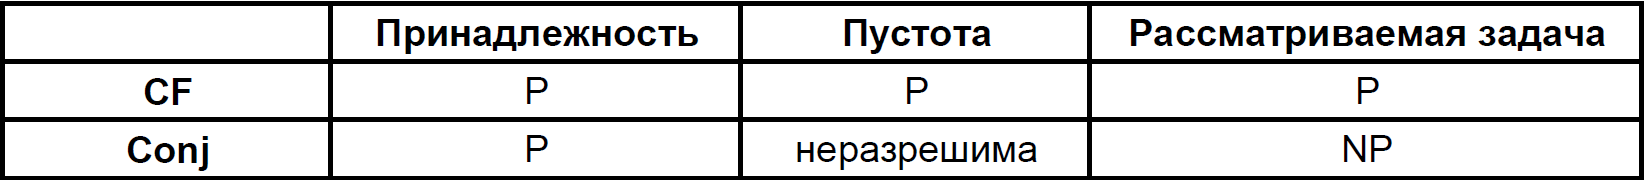
\includegraphics[width=12cm]{pictures/azimov-spbu-okhotin_tab1.png}
 \label{azimov-spbu-table}
\end{table}
